\chapter{Conclusion and Interesting Directions}
\label{chap:future}

In this dissertation, we investigated the use of neural networks as digital representations of media objects in multiple resolutions. Neural networks offer a model to approximate continuous functions, bridging the gap between the mathematical universe of modeling and the implementation universe, in the paradigm of the four universes. 

The current scenario where specific hardware as neural engines are being designed and comercilaized for consumer products as laptops, smartphones, smartwatches, VR headsets or even AR glasses, we believe that neural assets will play an important role in multiple industries.  In particular, we envision a future where neural networks will be standard digital representations of assets for particular applications in the audiovisual or games indutries. In that sense, we contributed with a representation that can fit the current rendering pipeline and is capable of encoding periodic material textures and even generating seamless textures under certain circunstances.


In this dissertation we have contributed to the understanding of the frequencies in sinusoidal neural networks and their connection to the multiresolution analysis theory. We have presented MR-Net as a family of architectures to encode signals in multiresolution showcansing its applications in media objects such as images and material textures. MR-Net is available as a software component, a flexible framework that implements the architectures described in Chapter \ref{chap:mr_snn} and the multiresolution training of the networks. It can be found in \cite{mrnetGithub}. Additionaly We demonstrated how to create periodic sinusoidal neural networks to represent periodic textures, we develop a techinique based on Poisson Equation to create seamless material textures, and we demonstrated how to use our architecture for rendering of textured objects.

Next, we explore some general limitations and interesting research directions related to our work.

% constituting what we call representational networks.

\section{Limitations}

\subsection{Frequencies}

By understanding the relationship between initialization of the first sinusoidal layer of a sinusoidal neural network and the frequencies learned by the model, we have made significant progress into connecting an emprirical hyperparameter to the Shannon-Nyquist theory. Moreover, we concluded that using integer frequencies is more appropriate as it has an underlying model that constitutes a representation for a well defined function space (periodic functions) and we can reduce the space of possible values for the initialiation to a discrete a finite set o values, thus helping on the design of a initialization strategy. 

However, there are two limitations that we believe should be addressed in future works. First, is that the frequencies of the first layer of the network need to be kep frozen 



\subsection{Implicit Functions}

Related to the frequencies choice, we would like to discuss the implicit represnetations of media, that is representing an object as a level set of an implicit function. We presented experiemnts for one-dimensional signals, that could be related to audio waves, and image signals. We have also experimented with higher order signals as it will be discussed in \ref{sec:3Dtextures}. However, all these media objects are represented explicitly as scalar or vector fields. In these cases, we can sample the signal uniformly and we have the support of the Shannon-Nyquist theory to guide our choices of initiaization of the networks.

For objects defined implicitly such as shapes given by a signed distance function or unsigned distance function, the relationship between the samples and the frequencies or even methods for filtering and building a multiscale representation are not straighforward. Works like MIP-PLICITS show that it is possible to and fruitful to decompose these signals and use a multistage network to represent them, but the terrain for choosing hyperparameters may be more unccertain.

Note that NeRF-based methods, that are usually referred as implicit do not fall in this category. Although they are not explicit representations of scenes, they are explicit representation of volume densities. The chalenge in this case comes from learning the volumetric function from 2D data.

\subsection{Compression}

Thinking of a useful digital representation we must make sure it is compact and lightweight to store in the disk or transmiti through the network. Part of this is due to small neural networks architectures, that is, managing to encode signals using networks with less weights. This part was a concern in this dissertation. However, this alone is not sufficient as the size of an image file is not only determided by the amaount of values it has to store, being either the total of pixels in a matrix or the total of weights in a network, but also by the level of compression.

In this sense, it is important to couple these results to efficient compression methods for neural networks such as \cite{dupont2021coin}, \cite{dupont2022coinpp} or even develop new methods for this goal.


\section{Interesting Directions}

\subsection{Volumetric Textures and Hypertextures}
\label{sec:3Dtextures}

3D textures also known as volumetric textures are defined and vector fields in the space. Solid textures offer practical advantages as they eliminate the need for computing $uv$-coordinates on a surface. We can apply it by directly verifyng the texture value at the coordinates $(x, y, z)$. 

Since they are represented explicitly in computer graphics, this looks like a natural extension of the discussion in Chapter \ref{chap:seamless-textures}. We have conducted preliminary experiments in this direction, using the Perlin Noise technique to generate procedural textures of materials like marble (Figure \ref{f:volumetric-texture}). We succcessfully trained a M-Net model to encode a volumetric texture and we managed to integrate it into the omniverse render (Figure \ref{f:volumetric-texture}). However, with this third spatial dimension, the network size increased greatly and we did not think it was worth it, specially in comparison to the procedural representation.

\begin{figure}[h]
   \centering
   \begin{subfigure}[b]{0.32\textwidth}
       \centering
       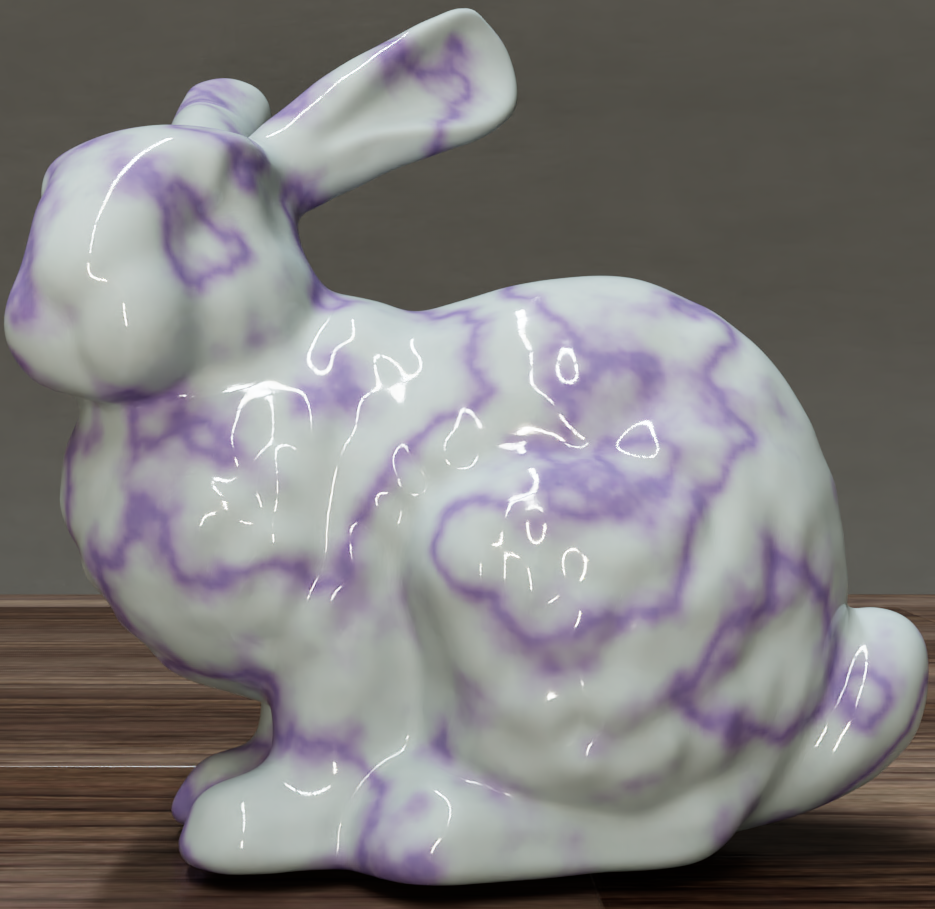
\includegraphics[width=\textwidth]{img/ch7/bunny_mrnet.0000.png}
       \caption{}
   \end{subfigure}
   \begin{subfigure}[b]{0.32\textwidth}
       \centering
       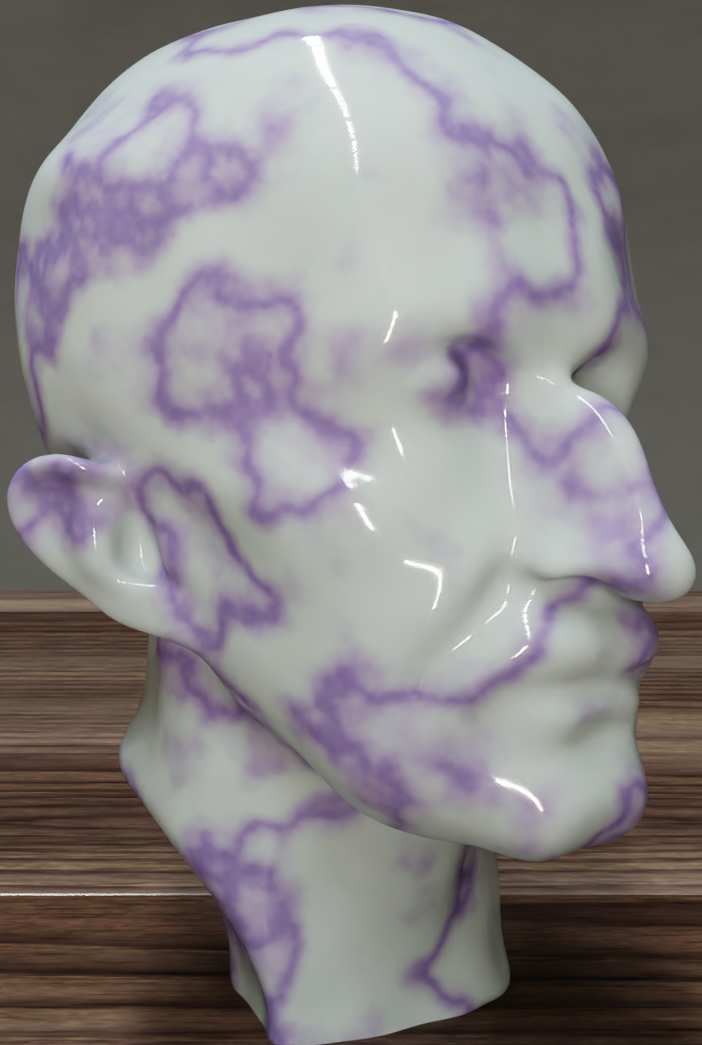
\includegraphics[width=\textwidth]{img/ch7/max_plank_mrnet_512_mc400.0099.png}
       \caption{}
   \end{subfigure}
   \begin{subfigure}[b]{0.32\textwidth}
       \centering
       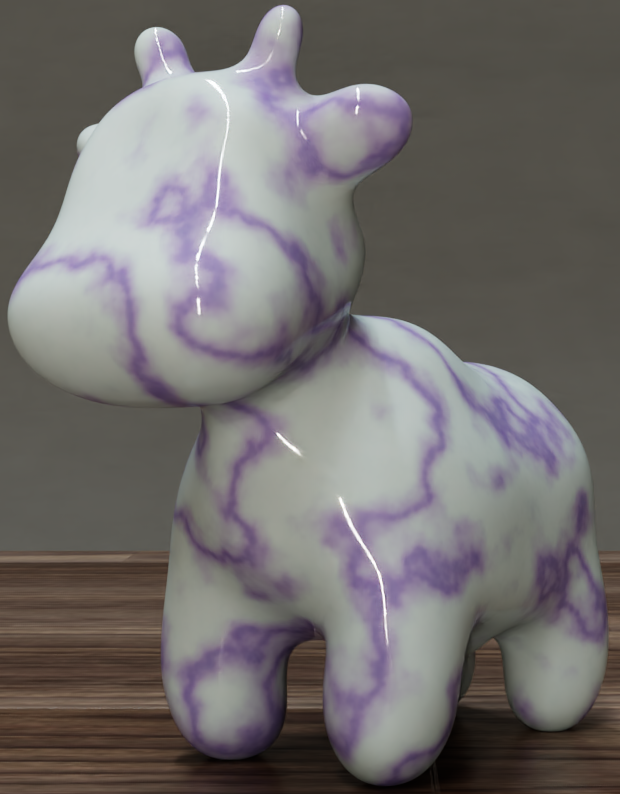
\includegraphics[width=\textwidth]{img/ch7/spot_mrnet.0101.png}
       \caption{}
   \end{subfigure}
   \caption{PLACEHOLDER}
   \label{f:volumetric-texture}
\end{figure}

One future research, thus, would be to investigate further how to optimize the training of MR-Net instaces in this case. Another promising research would be to generate a volumetric texture based on a 2D pattern. The ideia is to design a loss function or add the minimal information necessary to optimize it without requiring a large dataset, pretty much how the seamless texture generation in Chapter \ref{chap:seamless-textures} works.

Another interesting and particular object in computer graphics are the Hypertextures~\citep{hypertexture}. These objects model phenomena intermediate between shape and texture by using space-filling applicative functions to modulate density. The model is essentially an extension of procedural solid texture synthesis, but evaluated throughout a volumetric region instead of only at surfaces. Having a neural representation of this kind of phenonema to address for example fur or hair may be a path to efficient representation of these delicate objects. leveraging the versatility of vector fields in combination with surface representations, holds great potential.


\subsection{Irregular sampling}

The input for the neural network is a discrete representation. In this sense, sampling is a way to create a representation of a function based on its values at certain points of the domain. We presented many results based on regular sampling or uniform sampling, for which we have the Shannon-Nyquist theory as support. However, there are many scenarios where irregular sampling may be desirable.

First, for objects defined implicitly as level sets of implicit functions, for example shapes given by signed distance functions, we may not have an easy mechanism to define regular sampling and generate samples with these properties. Thus, irregular sampling is the default in this scenario.

Besides that, even in a scenario where we havean explicit representation of a signal, for example the one-dimensional signals we used in Chapter \ref{chap:sinusoidal}, it is evident that some points are features more important than others. For example, the critical points, those of maxima and minima (or saddle in higher dimensions) or inflection points are very relevant features for signal encoding. For this reason, we could decide to intentionally look for these points and maybe even use higher orther features like the derivatives to train a representational model of this signal. Moreover, thinking in terms of multiresoltion, we could have a stratified staregy of sampling.Furthermore, we believe that the capacity-based level of detail could benefit greatly of an irregular sampling scheme like, for example, the Poisson disk sampling \citep{stochastic_cook}.


In \citet{spectralPoster24} an ideia of using periodic neural networks to encode equirectangular panoramas is presented. In this case, there's a inherent challenge of dealing with the nature of this spherical representation that is periodic in one direction, but not in its orthogonal direction.  Besides, we believe it is possible to derive efficient representations of panoramas like this by leveraging an adaptive sampling grid as in Figure \ref{f:inr-panorama}, taking into account the fact that the equirectangular representation is oversampled in the poles.

When dealing with irregular sampling, we do not have aliasing, but we may have noise. Having a mechanism of filtering or not producing this noise when training the representational model is an interesting research direction.

\begin{figure}[!ht]
   \centering
   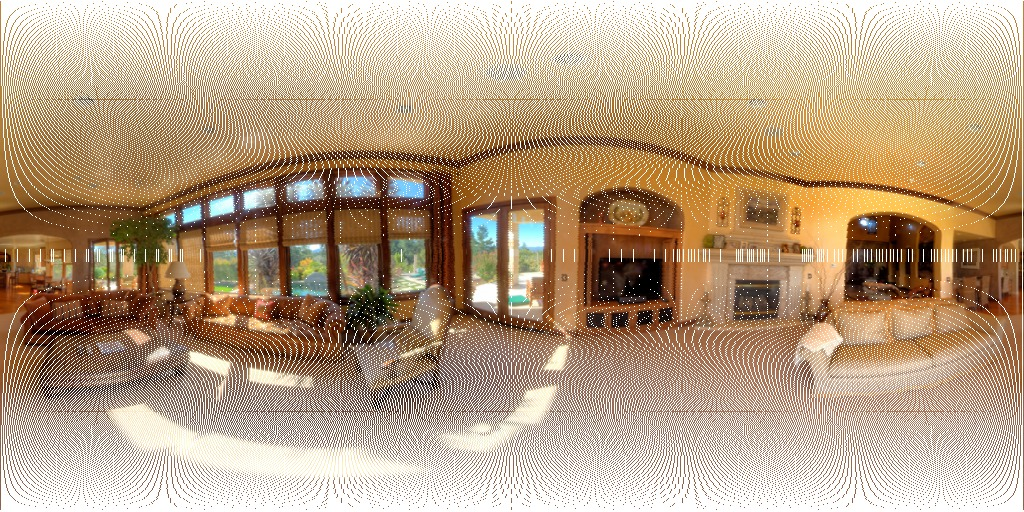
\includegraphics[width=0.80\linewidth]{img/ch7/sampling-pattern.jpeg}
   \caption{Sampling pattern for equirectangular panorama} 
   % \Description[Metric-aware sampling pattern for equirectangular panorama]{Metric-aware sampling pattern for equirectangular panorama}
   \label{f:inr-panorama}
\end{figure}


\subsection{Parameterizing Operations}

Up until now, we have focused exclusively on representing the media objects as a whole, providing a neural representation for them. 

An important step towards fully integrating neural networks as primitives in a graphics pipeline is the development of methods for operating and editing them. The functional structure of sinusoidal neural networks provides opportunities to explore algebraic structures for network manipulation. 


However, neural networks may be used to represent transformations in a space too. For instance, \cite{schardong2024neural} used sinusoidal neural networks to represent images of faces of people and also to parameterize morphing transformations between pairs of people so that it is possible to generate a third face that combines features of both individuals in a controlled manner.


We may go a step further a think that a media content may be interpreted as a single piece or decomposed in multiple subparts. For example we could represent a character moving in a scene as a video or as a sparse set of images and specific transformations between them. This may be lead to a storage efficient way of encoding some videos. Regressing a little bit, this strategy could be used in the sense of optical flow \citep{alfarano-opticalflow} to provide a general neural video format.


\section{Final Reflection}

Lore Ipsum!

% We have described a flexible method of working with signals in multiresolution in terms of multiple ways of preparing the input data, defining the MR-Net subclasses, and training multi-stage networks. In the applications presented in Sec. \ref{s:img}, we have explored a subset of this framework, showing cases where it improves upon existing state of the art techniques. Regarding other aspects of this groundwork, we have ongoing research on signal reconstruction from stochastic sampling, and training of L-Net models using the Laplacian pyramid, which may lead to novel imaging applications.  Some of the motivation and experiments with 1D signals in these directions are documented in \citet{supplemental}.


% In terms of future work, we plan to expand this research in two main directions. On one hand, we would like to explore the MR-Net architecture for other image applications including super-resolution, operations in the gradient domain, generation of periodic and quasi-periodic patterns, as well as image compression.
% On the other hand, we would like to extend the MR-Net representation to other media signals in higher dimensions, such as video, volumes, and implicit surfaces.